\section{Die Landschaft der Corona Dashboards}
TODO

\subsection{Dashboard – Ein Begriff mit Ursprung in der Automobilindustrie}
Im Kontext dieser Arbeit wird unter dem Begriff Dashboard die Definition von Duden verwendet. Duden definiert ein Dashboard als: \textbf{Ein Computerprogramm das relevante Informationen zusammenfasst und übersichtlich darstellt} ~\citep{term_definition_dashboard}.


\subsection{Webbasierte Corona Dashboards}
TODO


\subsubsection{Aufbau und Komponenten von webbasierten Dashboards}
Webbasierte Dashboards sind Dashboards, welche über das Internet zugänglich gemacht werden und mit Hilfe eines Webbrowsers dargestellt werden können. Wie herkömmliche Webseiten funktionieren auch webbasierte Dashboards nach dem \textit{Client-Server-Modell} (siehe Abbildung 6). Hierbei sendet der Browser (PC, Smartphone etc.) beim Besuch einer Internet Seite (\url{https://www.covid19.admin.ch/en/overview}) eine Anfrage an den Web Server. Dieser wiederum Antwortet mit dem gewünschten Inhalt (Corona Dashboard). Jedoch benötigt es noch eine dritte, sehr zentrale Komponente, die Datenquelle. In der heutigen Zeit sind Internet Seiten keine starren Textkonstrukte mehr, sie passen sich dynamisch an die Anforderungen des Nutzers an. Besonders für webbasierte Corona Dashboards sind dynamische Daten von enormer Bedeutung. 

Grundsätzlich wird für webbasierte Dashboards mindestens folgende Komponenten benötigt:
\begin{itemize}
    \item Web Server auf welchem die eigentliche Web Applikation läuft und welcher Anfragen entgegennimmt
    \item Datenbank auf welcher die Daten vorhanden sind
    \item Schnittstelle zwischen Datenbank und Webserver, welche die Kommunikation dieser beiden Komponenten ermöglicht
\end{itemize}

\subsubsection{Vorteile}
Ein grosser Vorteil von webbasierten Dashboards besteht in der grossen Erreichbarkeit der Nutzer. In der heutigen Zeit besitzen die meisten Personen nebst einem Computer ebenfalls über ein Smartphone mit integriertem Browser. Somit ist der Zugriff auf ein webbasiertes Dashboard nebst dem Computer auch über das Smartphone, über ein Tablet etc. möglich. Dies ist von enormer Bedeutung, da man so ortsunabhängig immer auf dem aktuellen Stand ist. Auch können moderne Web Applikationen Gebrauch vom GPS System des Smartphones machen und so standortbezogene Daten liefern. Die Voraussetzung hierzu ist lediglich die Nutzung eines modernen Browsers.

\begin{figure}[ht]
	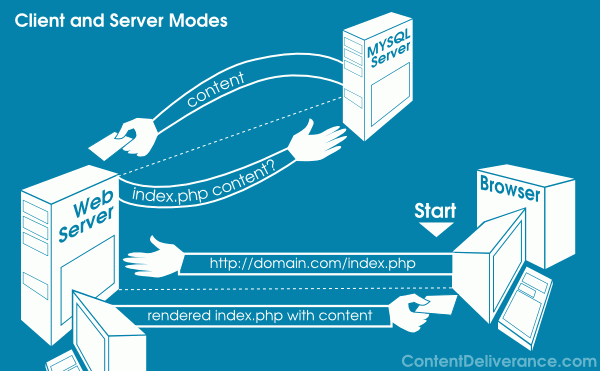
\includegraphics[width=12cm]{images/client_server_model.png}
	\centering
	\caption{Client-Server-Modell ~\citep{client_server_model}}
\end{figure}